\chapter*[INTRODUÇÃO]{Introdução}
\addcontentsline{toc}{chapter}{INTRODUÇÃO}
Atualmente, os smartphones são itens indispensáveis à vida em sociedade, já que possuem diversas funcionalidades que facilitam tarefas do cotidiano, como acessar internet, tirar fotos, encontrar lugares, etc. Dentre elas, o GPS\footnote{The Global Positioning System (GPS) is a U.S.-owned utility that provides users with positioning, navigation, and timing (PNT) services. \cite{u.s._government_gps.gov:_nodate}} se faz presente nos dispositivos móveis de maior popularidade, \citeonline[p.~12]{marcarini_utfpr_2015} afirma que os aparelhos eletrônicos com GPS tiveram grande crescimento de usuários nos últimos anos. Com isto em mente, este trabalho propõe a extensão da plataforma web já existente denominado Cidadão do Vale para um aplicativo de smartphone, e assim viabilizar uma melhor comunicação entre a prefeitura de Almenara-MG e os cidadãos, por meio da coleta de informações precisas sobre as questões urbanas da cidade de Almenara, e também do seu contexto regional.

A plataforma, Cidadão do Vale é uma configuração do framework ClickOnMap implementada em 2017 no IFNMG-Almenara em parceria com a Prefeitura Municipal, que permite o envio de informação sobre a existência de problemas relacionados à infraestrutura urbana. Desde o início do seu funcionamento, a plataforma contou com mais de mil contribuições públicas que, entre outros, revelou o perfil e distribuição espacial das principais reclamações, e apresentou-se como alternativa viável à gestão urbana da cidade.

Soluções como a em curso compõem um fenômeno multidimensional associado a um novo paradigma tecnológico de circulação de informações. Este novo padrão ocorre por meio da coleta de informações voluntária dos cidadãos, este conceito é denominado Informação Geográfica Voluntária (VGI)\footnote{Em inglês, Voluntereed Geographic Information.}, nas palavras de \citeonline[p.~vii]{costa_enriquecimento_2018} o VGI é como “uma espécie de informação com posicionamento geográfico que é coletada e/ou compartilhada voluntariamente pelos usuários por meio da Internet”.

É inegável que a internet se tornou uma das principais fontes de acesso à informação global, e o uso de aplicativos moveis são tendências em tecnologia no varejo. \citeonline{agencia_ibge_noticias2018}, mostra que o celular é o aparelho mais utilizado para a acessar à Internet (97,2\%) no total, o smartphone está presente em 46,7 milhões dos domicílios, além disso 38,6\% o utiliza como única forma de acesso à internet, o computador aparece em mais da metade (57,8\%), mas apesar disso seu uso é de apenas 2,3\%, pode-se notar que na Figura \ref{fig:internet} existem variações entre grandes regiões. Tais informações revelam a importância dos aplicativos para dispositivos móveis como meio de comunicação da população.
 \begin{figure}[H]
 	\centering
 	\caption{Percentual de domicílios brasileiros com acesso à Internet, segundo o equipamento utilizado.(2016)}
 	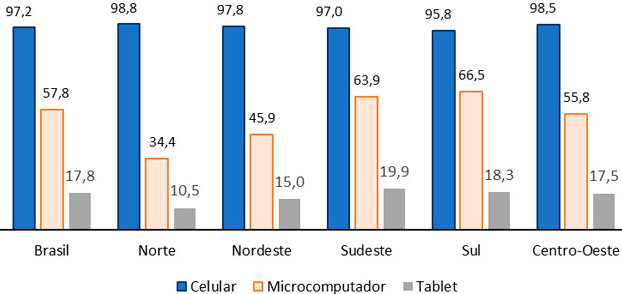
\includegraphics[width=0.6\linewidth]{Imagens/grafico}
	\legend{Fonte: \citeonline{agencia_ibge_noticias2018}}
	\label{fig:internet}
 \end{figure}

Ambientes urbanos são os espaços de produção e reprodução da vida social e onde as oportunidades de trabalho, educação, saúde, cultura, lazer e todas outras dimensões da vida cotidiana se concentram. O \citeonline[p.~19]{IBGEIBGE2011} define este termo como, "área legalmente definida como urbana, que se caracteriza por construções, arruamentos e intensa ocupação humana". Estes espaços vêm aumentando constantemente, como podemos ver na Figura \ref{fig:urban} abaixo.
\begin{figure}[H]
	\centering
 	\caption{Grau de urbanização, segundo as Grandes Regiões 1991/2010.} 
 	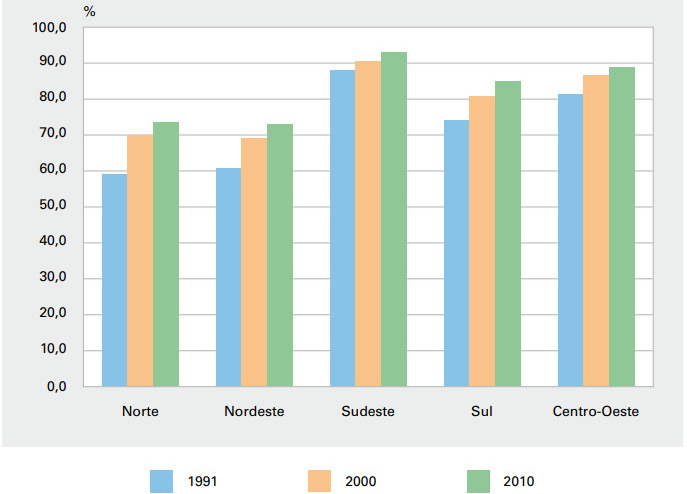
\includegraphics[width=0.6\linewidth]{Imagens/grafico2}		
	\legend{Fonte: \citeonline[p.~46]{IBGEIBGE2011} }
	\label{fig:urban}
\end{figure}  

O cenário atual de comunicação da população com o poder público não é centralizado, sendo a criação de um sistema para dispositivos moveis como o Cidadão do Vale uma alternativa via sistema informacional que possibilita essa centralização, organização e georreferenciamento das informações. O emprego de um sistema mobile, associado aos conceitos de VGI, facilita a comunicação entre as pessoas e a gestão municipal ao proporcionar um veículo de trocas que contêm dados objetivos, disposição das informações de forma pública, com possibilidade, inclusive, de pesquisas sobre a situação do município.


\section*{Objetivo Geral} 
Facilitar o gerenciamento dos problemas na infraestrutura em Almenara — MG, por meio do desenvolvimento de um sistema Android baseado no Cidadão do Vale.
	
\section*{Objetivos Específicos}
\begin{flushleft}
	Como objetivos específicos pretende-se:
\end{flushleft}

\begin{itemize}
	\item Definir modelo para desenvolvimento de software;
	\item Levantar requisitos do sistema web Cidadão do Vale;
	\item Elaborar projeto do sistema;
	\item Criar protótipo;
	\item Realizar o desenvolvimento do aplicativo Cidadão do Vale;
\end{itemize}

\section*{Justificativa}
A proposta justifica-se pela possibilidade de eliminação da necessidade de pesquisas de data fixa, onerosas ao poder público, já que o sistema web viabilizará o fluxo de informações continuas, consequentemente, de resoluções. A manutenção de um canal público capaz de centralizar as informações sobre a infraestrutura urbana em ambiente WebGIS e a visualização integrada ao território almenarense poderá auxiliar no processo de tomada de decisões e facilitar o diálogo entre a população e a gestão pública. Tais iniciativas geram impactos positivos sobre o orçamento público e democratizam o acesso à informação sobre a gestão do espaço urbano, e reafirmam o compromisso do IFNMG previsto na Lei nº. 11.892/08 \citeonline{LILDS2008}, de “orientar sua oferta formativa em benefício da consolidação e fortalecimento dos arranjos produtivos, sociais e culturais locais, identificados com base no mapeamento das potencialidades de desenvolvimento socioeconômico e cultural no âmbito de atuação do Instituto Federal”.